\chapter{Literature Review}
The following literature review section highlights the existing work that is related to our research. The work reviewed mostly consists of FAQ Processing and NLP techniques.

One of the caveats of the existing work is that, most of FAQ processing related work are based on the use on non-engineering fields such as the medical field. Likewise, since our research primarily focuses on the software engineering field, we hope to migrate any intuition that we can get from the existing work to our research. Therefore a certain degree of reading has been done in terms of handling technical languages and terminologies.

\pagebreak
\section{FAQ Processing}
FAQ retrieval is a crucial task when it comes to question answer pairs rankings \cite{faq_gen_1}. It is a process of retrieving the most relevant questions from a large collection of questions based on a user query. Achieving excellent performance in this task will solve many problems that we've discussed in the previous chapter \ref*{ch:problem_statement}. However, most of the traditional methods for FAQ generation are based on the use of extensive manual classification and software engineering \cite{faq_gen_1}, this method takes tremendous amount of time and effort to be done. This was particularly highlighted by \cite{10.1007/978-3-319-18356-5_30} \cite{5615722} \cite{6227139} \cite{7817112}. In addition, the performance of the framework is also affected by the quality of the manual classification and software engineering.

To address the issues brought-up, there are attempts and researches that have done to improve the predecessor. One of the approaches on solving the problem, is to automate the process of FAQ generation using NLP techniques. \cite{faq_gen_1} has made progress on using deep learning methods such as combining both Deep Matching Networks and Multihop Attention Networks in performing FAQ retrieval. Deep Matching Network also known as (DMN) is a deep learning model that generates a matching scores based of 2 matrices inputs. The matrices are made of the dot product of embeddings of every word of question with every word of answers.While Multihop Attention Networks on the other hand is proven to be effective for reasonings tasks like question answering, which is our focus in this paper \cite{faq_gen_1}. The network uses multiple "hops" of attention to gather information from a given input and make a prediction. It starts by encoding the input and then uses a decoder network that iteratively attends to different parts of the input, in order to generate an output.

\cite{10.1007/978-3-319-18356-5_30} \cite{10.1145/1099554.1099571} takes an approach where a whole architecture is designed to achieve Auto-Faq-Gen which includes scraping, question construction, a ranking algorithm, and the question generation. The architecture is shown in Figure \ref{auto-faq-gen-arch}.

\begin{figure}[H]
  \noindent 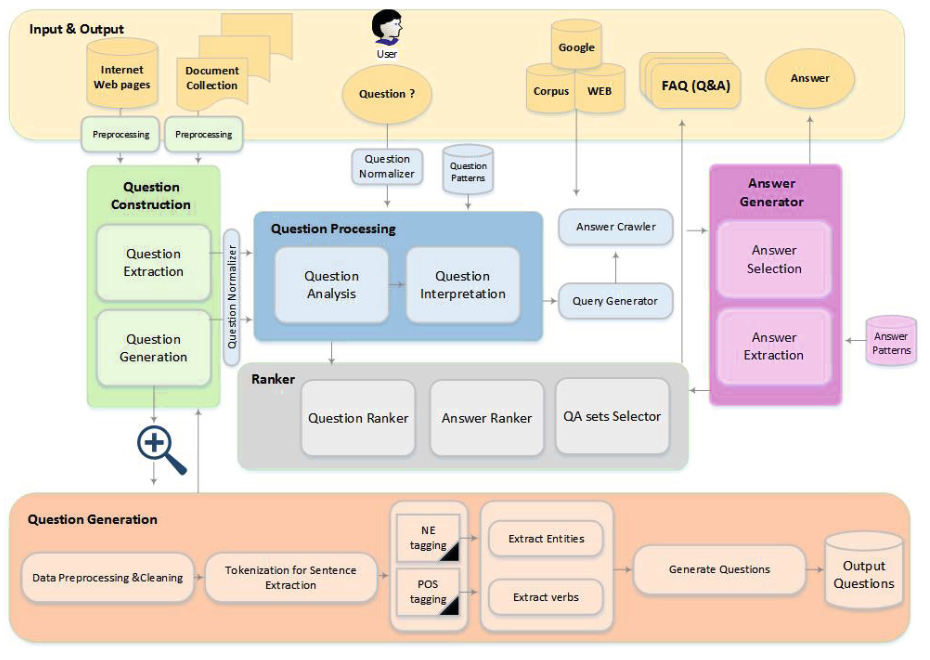
\includegraphics[scale=0.87]{assets/auto-faq-gen-architecture.png}
\caption{Auto FAQ Gen Architecture by \protect\citeA{10.1007/978-3-319-18356-5_30}}\label{auto-faq-gen-arch}
\end{figure}

The architecture presented was shown to be able to make Question and Answer Generation, Question Processing and a Ranker to rank answers.

\pagebreak
\subsection{Open Source Forums}
Open source forums are great sources of information for users to find answers to their questions. However, over time, most forums are bloated with a large number of posts, it's always easier if some form of ranking can be performed on these forums to improve user experience.  

\cite{5615722} \cite{10.1007/978-3-319-42911-3_25} has made progress in selecting, weighing, clustering and ranking contextual keywords in order to achieve questions abstraction and ultimately enhance the process of finding questions and related answers in open source forums. The author then proposed the solution to be in a format of semi-automatic FAQ generation.

\pagebreak
\subsection{Neural Networks}
Neural Networks are a collection of algorithms modelled after the human brain. It is a collection of algorithms used to identify patterns. It is able to learn independently by evaluating unstructured material with the capabilities of self-learning and adjusting weights to reach the optimal outcome.

Convolutional neural networks (CNN) and RNN has paved it's way towards text processing tasks for the past decade. In \cite{duan-etal-2017-question}, CNN was proposed as a method to handle questions generation based on a given passage, it was done in a retrieval based format while RNN was propose to perform questions generation with a generation-based method. Both neural network were able to pull off question pattern prediction, question topic selection, question ranking and lastly question generation. The proposed model is shown to be able to outperform the traditional methods such as MAP or MRR.

\pagebreak
\subsection{Context Matching} \label{lit:context_matching}
Another issue arises, where most of the time, the questions asked by the user might not be easily classified to fit with the existing questions in the FAQ database. This is because the questions asked by the user might be in a different form or context \cite{10.1007/978-3-319-42911-3_25}. For example, the question asked by the user might be in a different language, or the question asked by the user might be in a different form. 

Grammatically, misspellings are another set of issue that we can forsee when it comes to building automated questions answerings, highlighted by \cite{sms_faq_retrieval}.

Context Matching is important when it comes to ranking the answers to the user query. The traditional way to score similarity is naive, where the score is calculated by levenshtein distance. \cite{8054419} However, this method is not effective when it comes to ranking the answers. This is because the levenshtein distance is not able to capture the semantic meaning of the words. Another concept comes to mind which is BOW, the bag of words model, \cite{Improving_question_retrieval_in_community_question_answering_using_world_knowledge} highlighted to us where, BOWs similarity matching algorithm can be used on processed text (stop words removal, stemming, etc) to calculate the similarity between the query and the answer, however similarly to levenshtein distance, BOWs is not able to capture the semantic meaning of the words, which will bring false conceptual similarity between the query and the answer.

Word knowledge or Word Embedding is one of the solution to the traditional similarity matching algorithm. \cite{Improving_question_retrieval_in_community_question_answering_using_world_knowledge} proposed a method that uses word knowledge to improve the similarity matching algorithm. The model stitch together a knowledge base to a word, which then constructs a knowledge table which consists of the raw words, Hypernyms, Synonyms and Associative concept of words. This solution breaks the traditional similarity matching algorithm, where the similarity is calculated by the semantic meaning of the words, instead of the raw words. \cite{OTHMAN2019485} has made progress on proposing a method called "WEKOS (Word Embedding, Kmeans
and COSine based method)". WEKOS (Word Embedding, Kmeans and COSine) is a new method for question retrieval. The word embeddings of a question are weighted and averaged to get an overall representation of the question. The continuous word representations are learned in advance using the continuous bag-of-words (CBOW) model. \cite{OTHMAN2019485} The cosine similarity is used to calculate the similarity between the average of the word vectors corresponding to the question and that of each existing question.

\pagebreak
\subsection{Rankings}
Deep Matching Network also known as (DMN) is a deep learning model that generates a matching scores based of 2 matrices inputs. The matrices are made of the dot product of embeddings of every word of question with every word of answers.

Multi-hop Attention Network on the other hand is proven to be effective for reasonings tasks like question answering, which is our focus in this paper \cite{faq_gen_1}. The network uses multiple "hops" of attention to gather information from a given input and make a prediction. It starts by encoding the input and then uses a decoder network that iteratively attends to different parts of the input, in order to generate an output.

In order to solve the issue of context misconception between the query and the faq. We can highlight the issue below. 

\begin{figure}[H]
  \centering
  \noindent \fbox{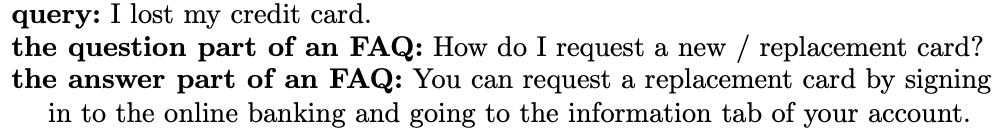
\includegraphics[scale=0.85]{assets/An_FAQ_search_method_query_issue.png}}
\caption{Misconception}\label{misconception_1}
\end{figure}

In the above example \ref*{misconception_1}, the query only matched with the correct output with 2 characters "I" and "Card", that way, the resulting score will be very low, even though the FAQ is relevant to the query. To counter this issue, the authors of \cite{10.1007/978-3-319-42911-3_25} proposed a method that predicts if the query corresponds to a FAQ using document classifier. The paper begins to highlight that the proposed document classifier uses binary classifiers to classifier each faq to the query. The sentences are broken into unigrams, bigrams to learn the dependency relation between the query and the faq.

\pagebreak
\subsection{Semantic Networks}
Automatically Generated Semantic Networks are networks that are generated by machine learning algorithms based on text or other forms of data. These networks are used to represent the relationships and connections between different concepts, entities, or topics in a structured manner, in order to facilitate various NLP or information retrieval tasks, such as classification, summarization, or question answering. They can be thought of as knowledge graphs constructed automatically from text.

Traditionally, QA (Question Answering) are managed using syntatic, semantic methods. However these methods are not pratical to perform well on low resource languages like Swahili. Semantic networks can be used to langauges like Swahili, where the language generally follows a subject-verb-object structure. \cite{9144082}.

\pagebreak
\subsection{Topic Modeling}
Topic Modeling is another great way to find Question and Answers Pairings. Topic modeling is a type of statistical modeling for discovering the abstract "topics" that occur in a collection of documents. It is a frequently used text-mining tool for discovery of hidden semantic structures in a text body. Latent Dirichlet Allocation (LDA) is a popular topic modeling technique that is used to discover topics in a collection of documents. LDA is a generative probabilistic model that assumes each document is a mixture of topics, and each topic is a mixture of words. The model is trained on a corpus of documents, and the topics discovered by the model can be used to label new, unseen documents. \cite{6227139}.

An architecture brought up by \cite{6227139} highlights the pipeline on leveraging topic modelling to perform prediction on the question and answer pairings. The pipeline proposed extracts the topics from the corpus, then the topics are used to label the questions and answers, which then extracts answers that closely relates to the topic mined by the model.

\pagebreak

\section{Stop Words}
Stop words are words that are filtered out before or after processing of natural language data (text). Though "stop words" usually refers to the most common words in a language, there is no single universal list of stop words used by all natural language processing tools. The stopwords used in technical languages differs from the general stopwords list used by general application such as the NLTK library \cite{stopwords_1} \cite{stopwords_2}.

The properties of stopwords can be defined as follows \cite{9074166}:
  \begin{itemize}
    \item Words used for connecting important words.
    \item Words that are not important to the meaning of the sentence.
    \item  Words that occurs frequently in the text.
  \end{itemize}


While it might be wise to perform stopwords removal tasks on tasks such as Information Retrieval (IR), classification, it is not advisable to perform stopwords removal on tasks like summarization. \cite{9074166}.

\cite{stopwords_1} addresses the gap in identifying stopwords for texts in software engineering fields which are not covered by the general stopwords list. The concluded stopwords list is statistically identified and evaluated by experts. 

Phrases can be detected by using the algorithm of Mikolov at al \cite{NIPS2013_9aa42b31}. The algorithm works by finding words that are frequently used together.

\[ score(wi, wj) = ((count(wi*wj) - S)|N| / count(wi) * count(wj)) \]

Term frequency-inverse-document-frequency (TFIDF) is a numerical statistic that is intended to reflect how important a word is to a document in a collection or corpus. Many information retrieval systems use TFIDF as a central tool.

TF (Term Frequency) is the number of times a word appears in a document, divided by the total number of words in the document. 

\[ TF = \frac{Number of times term t appears in a document}{Total number of terms in the document} \]

IDF (Inverse Document Frequency) is the log of the number of the documents in the corpus divided by the number of documents that contain the word w.

\[ IDF = log_e(\frac{Total number of documents}{Number of documents with term t in it}) \]

Term frequency-inverse-document-frequency (TFIDF) is then the product of TF and IDF.

\[ TFIDF = TF * IDF \]

This method particularly favours words that appear many times in a document. Both of this methods are used to score and rank words in a document, and potentially form a stopwords lists. An interesting fact is that with using the two methods mentioned above, the stopwords list can be generated for a specific domain. 

\pagebreak 

\section{Sentiment Analysis}
Sentiment analysis is the process of determining whether a piece of writing is positive, negative, or neutral. It's also known as opinion mining, deriving the opinion or attitude of a speaker. A common use case of sentiment analysis is to discover how people feel about a particular topic. For example, sentiment analysis can be used to discover how people feel about a new movie, or to learn about the general sentiment towards a new product.

While most sentiment analysis work are based of current social medias such as Twitter, Facebook, and Instagram, sentiment analysis can be applied to any text. For instance, \cite{ABSAUSGRD2019} uses sentiment analysis to further investigate and understand the customers needs and wants for goverment entities.

\subsection{Grananularity}
Sentiment analysis can be performed on different levels of granularity. The level of granularity refers to the level of detail at which the sentiment is expressed. There are three levels of granularity: sentence-level, document-level, and aspect-level. Taking into account the level of granularity is important because it affects the type of sentiment analysis that can be performed, and the type of results that can be obtained \cite{ABSAUSGRD2019}.

\subsection{Aspect Based}
Aspect-Based Sentiment Analysis (ABSA) is a subfield of sentiment analysis that focuses on identifying and extracting opinions towards specific aspects or features of an entity such as a product, a service, or a person. It involves analyzing a piece of text to determine the sentiment expressed towards a particular aspect, rather than the overall sentiment of the text. This type of analysis is useful in understanding the specific opinions and attitudes of customers and users towards a particular product or service, and can be used in a variety of applications such as customer service, market research, and product development \cite{ABSAUSGRD2019} \cite{9260162} \cite{xue-li-2018-aspect} \cite{MABDELGWAD20226652}.

The goal of aspect-based sentiment analysis is to identify the sentiment expressed towards a particular aspect of an entity. For example, consider the following sentence: 

\noindent \begin{lstlisting}
"The food at this restaurant is great, but the service is terrible."
\end{lstlisting}
\captionof{lstlisting}{Example of Aspect-based Sentiment Analysis}

\noindent In this sentence, the overall sentiment might be positive, but in actuality the sentiment towards the food is positive, while the sentiment towards the service is negative. Therefore by using Aspect-based sentiment analysis can be used to identify the sentiment towards the food and the service separately. \cite{ABSAUSGRD2019} took this intuition and applied it to the government sector. They used the ABSA to identify the sentiment towards the government services and the government entities.

\noindent In our research, we'll be using the ABSA model in the hopes where it'll improve the FAQ Ranker in terms of ranking their sentiment to potentially indicate the quality of the answer.

\subsection{Traditional Methods}
Lexicon and Corpus based approaches are unsupervised learning methods to understand the sentiment of a text. The lexicon based approach uses a predefined list of words coupled with the annotated polarity values of the word's sentiment. This approach has a major downside where there might be numerous words and expressions that are not included in the lexicons. 

Corpus based approach however focuses more in predicting the word to be a prefixer or suffixer of the sentiment word. This approach is more accurate than the lexicon based approach, but it is still not perfect. \cite{SOABSAUMLT2021}
\subsection{Machine Learning and Deep Learning}
Multiple researches has proven that machine learning can make promising results in terms of ABSA specifically polarity classification. It was highlighted that attention-based or non attention based LSTM models can be used to achieve promising results \cite{SOABSAUMLT2021} \cite{9260162}

\noindent SVM had received the highest popularity in terms of polarity classification, it was often used with association rules and feature selection such as PCA to achieve promising results \cite{SOABSAUMLT2021} \cite{Zainuddin2018HybridSC} \cite{AlSmadi2017DeepRN}

\noindent Convolutional Neural Network were also used to predict polarity of a sentence, there were a handfull of attempts in using CNN coupled with Word2Vec that had been proven to be effective \cite{SOABSAUMLT2021} \cite{ABSAUDNASO2020} \cite{Rezaeinia2019SentimentAB} \cite{10.1016/j.neucom.2019.04.038} 

\noindent To learn long term associations and dependencies between texts in a sentence or a document. Long Short Term Memory (LSTM) was a popular choice in learning information dependencies across the history of sentences in a document. Multiple atempts had been made to take advantage of LSTM models in buildling polarity classification models \cite{he-etal-2018-exploiting} \cite{10.1016/j.future.2018.10.041} \cite{Sindhu2019AspectBasedOM} 

\pagebreak

\section{Summarization}
Text summarization is the process of automatically generating a shorter version of a text that preserves the most important information. There are two main types of text summarization: extractive and abstractive. Extractive summarization involves selecting and concatenating important sentences from the original text, while abstractive summarization involves generating new sentences that summarize the meaning of the original text \cite{ATSMACR2022} \cite{ATSUSTSRAB2016}.

In contrast to general text summarization, summarizing software engineering related texts differs itself from the general text summarization. The main difference is that the software engineering related texts are often more technical and contain more technical terms, not to mention that at times, processing raw source codes can be a challenge \cite{8449647}.

The evaluation metrics used generally is to calcualate the compression rate denoted by the ratio of the length of the summary to the length of the original text.\cite{ATSMACR2022} The formula is as follows:
 
\[ Compression Rate = \frac{Length of Summary}{Length of Original Text} \]

\pagebreak
\subsection{Extractive Summarization}

Extractive summarization involves selecting and concatenating important sentences from the original text. The most common approach to extractive summarization is to use a sentence ranking model to rank sentences in the original text, and then select the top ranked sentences to form the summary. The sentence ranking model can be trained using a variety of features, such as the number of named entities in the sentence, the number of words in the sentence which closely relates to TFIDF, the number of words in the sentence that are also in the original text, and the number of words in the sentence that are also in the summary \cite{ATSMACR2022}.

CN-Summ is one of the notable extractive summarization model that was introduced by \cite{ACNATTS2009}. CN-Summ is a neural network based model that uses a graph-like architecture to connect sentences that shared common significant nouns. The model consist preprocesses, a graph construction, and finally selecting the first x sentences as the summarization.

Similarly to using LDA in sentiment analysis \cite{SOABSAUMLT2021}, LDA has also shed light in the field of extractive summarization. \cite{ATSULSA2011} proposed the use of LDA to extractive summarization. The model uses LDA to extract the most important topics in the original text, and then uses the topics to rank sentences in the original text. 
\pagebreak

\subsection{Abstractive Summarization}
Abstractive summarization involves generating new sentences that summarize the meaning of the original text. The most common approach to abstractive summarization is to use a sequence to sequence neural network to generate the summary. A sequence to sequence neural network such as RNN, LSTM is used because they are well-suited for processing sequences of data, such as text. The recurrent connections in RNNs allow them to maintain a hidden state that can capture information from previous steps in the sequence, which is useful for keeping track of contextual information as the model reads the input text. This allows the model to generate a summary that is both concise and semantically relevant to the input text \cite{ATSMACR2022}. 

AMR (Abstract Meaning Representation) was one of the RNN based methods that was introduced by \cite{banarescu-etal-2013-abstract}. AMR is a neural network based model produces a single graph to represent time series information in the text to form an abstractive summary. 

ATSDL is another attempt where the paper introduce a use of combining advantages of extractive and abstractive summazy to form a hybrid model. The model uses a sequence to sequence neural network to generate the summary, and then uses a sentence ranking model to rank the sentences in the summary. The top ranked sentences are then selected to form the final summary \cite{ATSMACR2022}. A phrase collection model called MOSP was introduced to generate and learn phrase representations and their relationships in a document, the model solves the problem of unusual terms, which abstrative models faced most of the time.

\pagebreak
\section{Evaluation Metrics}
Evaluating the success rate of extracting FAQ can be subjective, not all datasets coincide with the same domain. Therefore, a manual evaluation approach are mostly used to evaluate the success rate of a question finding process \cite{10.1145/1099554.1099571}. Manual classification of the questions pairs are carried out and the results are compared with the results of the question finding process.

However there are semi-automated frameworks that can potentially be used to evaluate the success rate of a question finding process. Alternatively, a user feedback framework can be constructed, where a user can provide feedback on the accuracy of the question finding process. The feedback can be used to evaluate the success rate of the question finding process \cite{10.1007/978-3-319-18356-5_30}.

\pagebreak
